\documentclass[tikz,border=8pt]{standalone}
\usepackage{amsmath,amssymb}
\usetikzlibrary{arrows.meta,calc,decorations.markings,decorations.pathmorphing,patterns,shapes.geometric,positioning}

\begin{document}
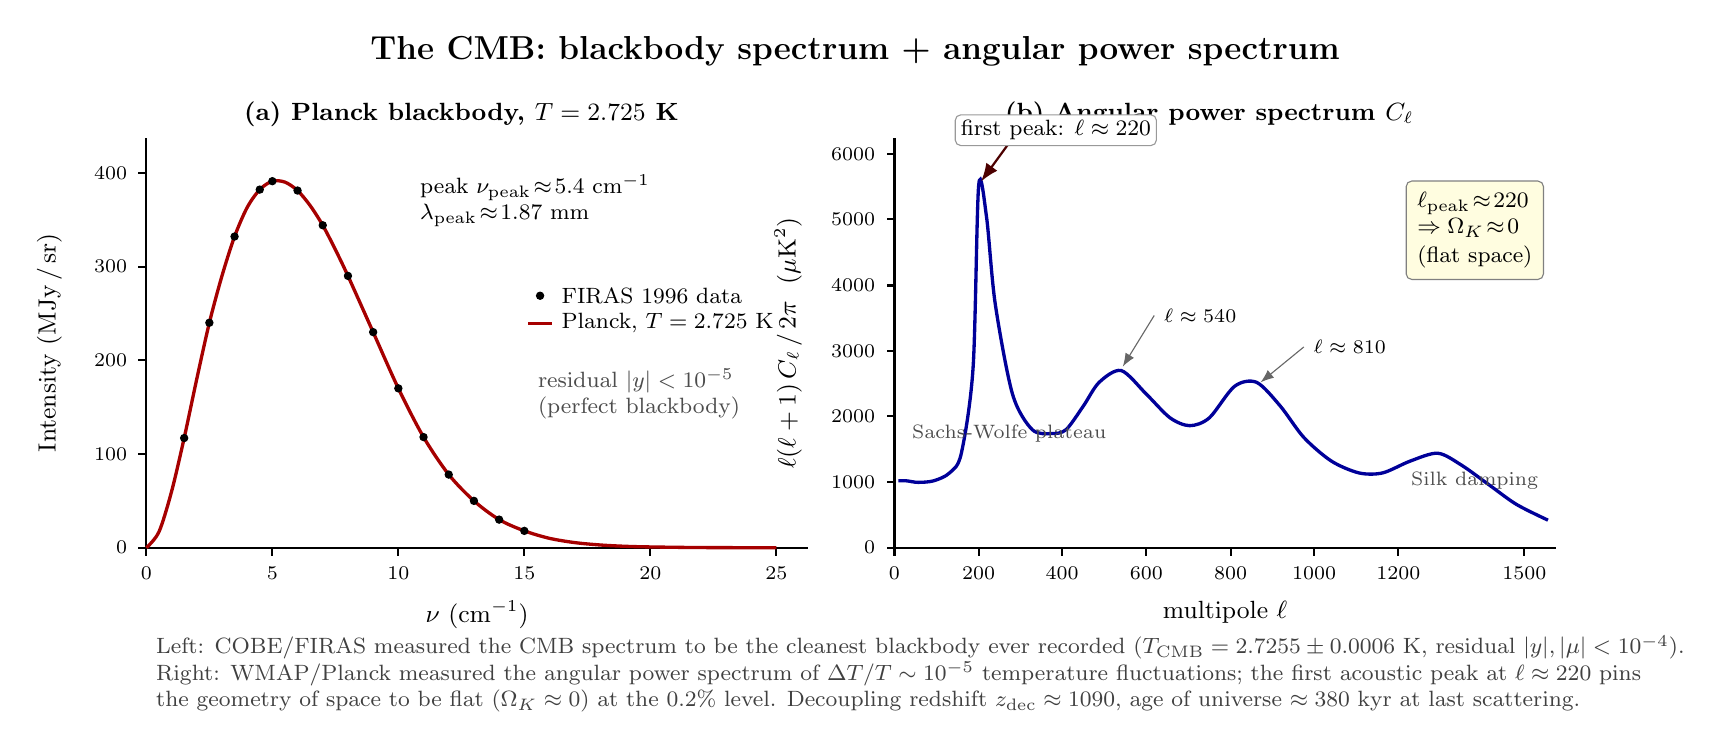
\begin{tikzpicture}[>=Latex,
  axisline/.style={draw=black, thick},
  ticklbl/.style={font=\scriptsize, anchor=north},
  yticklbl/.style={font=\scriptsize, anchor=east},
  planckcurve/.style={draw=red!65!black, very thick},
  datapt/.style={circle, fill=black, draw=black, inner sep=0pt, minimum size=2.6pt},
  cellcurve/.style={draw=blue!60!black, very thick}]

  % --- Overall title -------------------------------------------------------
  \node[font=\large\bfseries, align=center] at (0, 6.3) {%
    The CMB: blackbody spectrum + angular power spectrum};

  % ========================================================================
  % LEFT PANEL: Planck blackbody at T = 2.725 K
  % Plot intensity B_nu(T) in MJy/sr vs wavenumber nu (cm^-1)
  % Range: nu = 0..25 cm^-1; intensity peak ~390 MJy/sr at nu ~ 5.4 cm^-1
  % We work in plot coords: x in [0, 8] cm  (nu 0..25 cm^-1)
  %                          y in [0, 5] cm  (intensity 0..420 MJy/sr)
  % ========================================================================
  \begin{scope}[shift={(-9.0, 0)}]

    % Panel title
    \node[font=\small\bfseries, align=center] at (4.0, 5.5)
      {(a) Planck blackbody, $T = 2.725$ K};

    % Axes box
    \draw[axisline] (0, 0) -- (8.4, 0); % x-axis
    \draw[axisline] (0, 0) -- (0, 5.2); % y-axis

    % x-ticks: nu = 0, 5, 10, 15, 20, 25 cm^-1  -> x = 0, 1.6, 3.2, 4.8, 6.4, 8.0
    \foreach \nu/\xc in {0/0, 5/1.6, 10/3.2, 15/4.8, 20/6.4, 25/8.0} {
      \draw[axisline] (\xc, 0) -- (\xc, -0.10);
      \node[ticklbl] at (\xc, -0.12) {\nu};
    }
    % y-ticks: I = 0, 100, 200, 300, 400  -> y = 0, 1.19, 2.38, 3.57, 4.76
    \foreach \I/\yc in {0/0, 100/1.19, 200/2.38, 300/3.57, 400/4.76} {
      \draw[axisline] (0, \yc) -- (-0.10, \yc);
      \node[yticklbl] at (-0.12, \yc) {\I};
    }

    % Axis labels
    \node[font=\small, anchor=north] at (4.2, -0.55) {$\nu$ (cm$^{-1}$)};
    \node[font=\small, rotate=90, anchor=south] at (-0.95, 2.6)
      {Intensity (MJy\,/\,sr)};

    % Planck curve (precomputed): wavenumbers nu (cm^-1) -> intensity B_nu (MJy/sr)
    % at T=2.725 K. Conversion: x = nu * 8/25, y = B * 5/420.
    % Sampled values (nu, B):
    %  0.5 -> 17, 1.0 -> 60, 1.5 -> 117, 2.0 -> 180, 2.5 -> 240, 3.0 -> 290,
    %  3.5 -> 332, 4.0 -> 363, 4.5 -> 382, 5.0 -> 391, 5.5 -> 390, 6.0 -> 381,
    %  6.5 -> 365, 7.0 -> 344, 7.5 -> 318, 8.0 -> 290, 9.0 -> 230, 10.0 -> 170,
    %  11.0 -> 118, 12.0 -> 78, 13.0 -> 50, 14.0 -> 30, 15.0 -> 18, 16.0 -> 10,
    %  17.0 -> 5.5, 18.0 -> 2.9, 19.0 -> 1.5, 20.0 -> 0.8, 22.0 -> 0.18, 25.0 -> 0.02
    \draw[planckcurve] plot[smooth] coordinates {
      (0.000, 0.000)
      (0.160, 0.202)
      (0.320, 0.714)
      (0.480, 1.393)
      (0.640, 2.143)
      (0.800, 2.857)
      (0.960, 3.452)
      (1.120, 3.952)
      (1.280, 4.321)
      (1.440, 4.548)
      (1.600, 4.655)
      (1.760, 4.643)
      (1.920, 4.536)
      (2.080, 4.345)
      (2.240, 4.095)
      (2.400, 3.786)
      (2.560, 3.452)
      (2.880, 2.738)
      (3.200, 2.024)
      (3.520, 1.405)
      (3.840, 0.929)
      (4.160, 0.595)
      (4.480, 0.357)
      (4.800, 0.214)
      (5.120, 0.119)
      (5.440, 0.065)
      (5.760, 0.035)
      (6.080, 0.018)
      (6.400, 0.010)
      (7.040, 0.002)
      (8.000, 0.000)
    };

    % FIRAS data points (a few representative samples on the curve;
    % real error bars are <50 nW/m^2/sr/cm^-1, invisible at this scale)
    \node[datapt] at (0.480, 1.393) {};
    \node[datapt] at (0.800, 2.857) {};
    \node[datapt] at (1.120, 3.952) {};
    \node[datapt] at (1.440, 4.548) {};
    \node[datapt] at (1.600, 4.655) {};
    \node[datapt] at (1.920, 4.536) {};
    \node[datapt] at (2.240, 4.095) {};
    \node[datapt] at (2.560, 3.452) {};
    \node[datapt] at (2.880, 2.738) {};
    \node[datapt] at (3.200, 2.024) {};
    \node[datapt] at (3.520, 1.405) {};
    \node[datapt] at (3.840, 0.929) {};
    \node[datapt] at (4.160, 0.595) {};
    \node[datapt] at (4.480, 0.357) {};
    \node[datapt] at (4.800, 0.214) {};

    % Annotation: peak label
    \node[font=\footnotesize, anchor=south west, align=left, fill=white,
          inner sep=2pt] at (3.4, 4.0)
      {peak $\nu_{\rm peak}\!\approx\!5.4$ cm$^{-1}$\\
       $\lambda_{\rm peak}\!\approx\!1.87$ mm};

    % FIRAS legend mark
    \node[datapt] at (5.0, 3.2) {};
    \node[font=\footnotesize, anchor=west] at (5.15, 3.2)
      {FIRAS 1996 data};
    \draw[planckcurve, line width=1.2pt] (4.85, 2.85) -- (5.15, 2.85);
    \node[font=\footnotesize, anchor=west] at (5.15, 2.85)
      {Planck, $T=2.725$ K};

    % Residual annotation
    \node[font=\footnotesize, anchor=west, text=black!70, align=left]
      at (4.85, 1.95)
      {residual $|y|<10^{-5}$\\
       (perfect blackbody)};

  \end{scope}

  % ========================================================================
  % RIGHT PANEL: angular power spectrum C_l vs l
  % x-axis: l from 0 to ~1500, log-ish on low-l, linear ok for sketch
  % y-axis: l(l+1)C_l/(2 pi) in (mu K)^2, peaks at ~5500 (first), ~2700, ~2400
  % Plot box: x in [0, 8] cm, y in [0, 5] cm
  % Map l: l=0 -> 0, l=200 -> 1.07, l=400 -> 2.13, l=800 -> 4.27, l=1500 -> 8.0
  % Map C_l: 0 (mu K)^2 -> 0, 6000 (mu K)^2 -> 5.0
  % ========================================================================
  \begin{scope}[shift={(0.5, 0)}]

    % Panel title
    \node[font=\small\bfseries, align=center] at (4.0, 5.5)
      {(b) Angular power spectrum $C_\ell$};

    % Axes
    \draw[axisline] (0, 0) -- (8.4, 0); % x
    \draw[axisline] (0, 0) -- (0, 5.2); % y

    % x-ticks (l): 0, 200, 400, 600, 800, 1000, 1200, 1500
    \foreach \l/\xc in {0/0, 200/1.07, 400/2.13, 600/3.20, 800/4.27, 1000/5.33, 1200/6.40, 1500/8.0} {
      \draw[axisline] (\xc, 0) -- (\xc, -0.10);
      \node[ticklbl] at (\xc, -0.12) {\l};
    }
    % y-ticks: 0, 1000, 2000, 3000, 4000, 5000, 6000  (mu K)^2
    \foreach \C/\yc in {0/0, 1000/0.83, 2000/1.67, 3000/2.50, 4000/3.33, 5000/4.17, 6000/5.00} {
      \draw[axisline] (0, \yc) -- (-0.10, \yc);
      \node[yticklbl] at (-0.12, \yc) {\C};
    }

    % Axis labels
    \node[font=\small, anchor=north] at (4.2, -0.55) {multipole $\ell$};
    \node[font=\small, rotate=90, anchor=south] at (-1.05, 2.6)
      {$\ell(\ell+1)\,C_\ell\,/\,2\pi$\ \ ($\mu$K$^2$)};

    % C_l curve (sketch of TT power spectrum):
    % Low-l Sachs-Wolfe plateau ~ 1000 (mu K)^2
    % First peak: l ~ 220, height ~ 5500 (mu K)^2
    % Trough: l ~ 410, height ~ 1700
    % Second peak: l ~ 540, height ~ 2700
    % Trough: l ~ 680, height ~ 1900
    % Third peak: l ~ 810, height ~ 2500
    % Damping tail decreases to ~ 100 by l ~ 2000
    \draw[cellcurve] plot[smooth] coordinates {
      (0.05, 0.85)
      (0.15, 0.85)
      (0.30, 0.83)
      (0.50, 0.85)
      (0.70, 0.95)
      (0.85, 1.20)
      (1.00, 2.30)
      (1.07, 4.60)
      (1.17, 4.20)
      (1.28, 3.10)
      (1.50, 1.95)
      (1.75, 1.50)
      (2.00, 1.45)
      (2.18, 1.50)
      (2.40, 1.80)
      (2.60, 2.10)
      (2.88, 2.25)
      (3.20, 1.95)
      (3.50, 1.65)
      (3.75, 1.55)
      (4.00, 1.65)
      (4.32, 2.05)
      (4.60, 2.10)
      (4.90, 1.80)
      (5.20, 1.40)
      (5.55, 1.10)
      (5.90, 0.95)
      (6.20, 0.95)
      (6.55, 1.10)
      (6.90, 1.20)
      (7.20, 1.05)
      (7.55, 0.80)
      (7.90, 0.55)
      (8.30, 0.35)
    };

    % Annotation arrows: first peak label
    \draw[->, thick, black!70!red] (1.5, 5.2) -- (1.10, 4.65);
    \node[font=\footnotesize, anchor=south, fill=white,
          inner sep=2pt, draw=black!40, rounded corners=2pt]
      at (2.05, 5.10) {first peak: $\ell\approx 220$};

    % Annotation: second/third peaks
    \draw[->, thin, black!60] (3.30, 2.95) -- (2.90, 2.30);
    \node[font=\scriptsize, anchor=west] at (3.30, 2.95)
      {$\ell\approx 540$};

    \draw[->, thin, black!60] (5.20, 2.55) -- (4.65, 2.10);
    \node[font=\scriptsize, anchor=west] at (5.20, 2.55)
      {$\ell\approx 810$};

    % Annotation: SW plateau and damping tail
    \node[font=\scriptsize, anchor=west, text=black!70] at (0.10, 1.45)
      {Sachs-Wolfe plateau};
    \node[font=\scriptsize, anchor=east, text=black!70, align=center] at (8.30, 0.85)
      {Silk damping};

    % Implication box at bottom-right
    \node[font=\footnotesize, anchor=south east, align=left, fill=yellow!12,
          draw=black!50, rounded corners=2pt, inner sep=4pt]
      at (8.25, 3.40)
      {$\ell_{\rm peak}\!\approx\!220$\\
       $\Rightarrow \Omega_K\!\approx\!0$\\[1pt]
       (flat space)};

  \end{scope}

  % --- Bottom legend / context --------------------------------------------
  \node[font=\footnotesize, anchor=west, align=left, text=black!75]
    at (-9.0, -1.6)
    {Left: COBE/FIRAS measured the CMB spectrum to be the cleanest blackbody ever recorded
     ($T_{\rm CMB}=2.7255\pm 0.0006$ K, residual $|y|,|\mu|<10^{-4}$).\\
     Right: WMAP/Planck measured the angular power spectrum of $\Delta T/T\sim 10^{-5}$
     temperature fluctuations; the first acoustic peak at $\ell\approx 220$ pins\\
     the geometry of space to be flat ($\Omega_K\approx 0$) at the $0.2\%$ level.
     Decoupling redshift $z_{\rm dec}\approx 1090$, age of universe $\approx 380$ kyr at last scattering.};

\end{tikzpicture}
\end{document}
